% class definitions
\documentclass[a4paper,12pt]{scrartcl}

% Packages

\usepackage[utf8]{inputenc}
\usepackage[ngerman]{babel}
\usepackage[T1]{fontenc}
\usepackage{graphicx}
\usepackage{lmodern}
\usepackage{tabto}
\usepackage{listings}
\usepackage{quoting} %
\usepackage{lipsum}
\usepackage[left, pagewise, edtable]{lineno}
\quotingsetup{font={itshape}, leftmargin=2em, rightmargin=0in, vskip=1ex}
\usepackage{framed} 
\usepackage{xcolor} 
\colorlet{shadecolor}{gray!25}

\newenvironment{myshaded}{\colorlet{shadecolor}{lightgray}\color{black}\begin{shaded}\begin{internallinenumbers}}{\end{internallinenumbers}\end{shaded}}


\usepackage[backend=biber, style=authoryear]{biblatex}
\addbibresource{quellen.bib}


% Front page

\title{ Flubot:\\ Android-Malware verbreitet sich über Fake-Patches }
\subtitle{Cybersecurity}
\author{Moritz Rupp}
\date{Wintersemester 2021/22}
\setlength{\parindent}{0em} 

% Mathepakete
\usepackage{amsfonts}
\usepackage{amsmath}

%Document start 
\begin{document}
 


\maketitle
\newpage
\tableofcontents
\newpage


\section{Abstract}
Die tägliche Nutzung von Smartphones ist seit nunmehr über 10 Jahren in der breiten Gesellschaft angekommen. Egal ob Kurznachrichtendienste, soziale Medien, online Banking oder Shopping. In allen Bereichen des sozialen und geschäftlichen Lebens findet das Smartphone Anwendung. Auch neuere Erscheinungen wie der Online-Handel mit Kryptowährungen finden größtenteils über mobile Endgeräte statt. \\
Derzeit sind laut statista\footnote{\cite{statista | 2021}} über 4 Milliarden mobile Geräte im Umlauf. Davon nutzen über 70 Prozent\footnote{{statista | 2021}} das Betriebssystem Android.
Diese enorme Anzahl an ähnlichen Geräten auf denen sensitive Daten laufen, bietet eine große Angriffsfläche für Cyberkriminelle.
Hierbei gilt Phishing seit Jahren als eine der größten Bedrohungen.
Meist wird versucht Login Daten durch Imitation eines Anbieters oder Dienstes abzugreifen.
Des Weiteren stellen Botnetze eine große Gefahr dar. Diese können 
automatisiert in kurzer Zeit tausende Geräte infizieren.\\
Der Banking Trojaner Flubot kombiniert Phishing Methoden und Botnetze, um sich großflächig zu verbreiten und sensible Daten abzufischen.\\ Diese Arbeit beleuchtet die Funktionsweise und technischen Hintergründe der Malware.



\newpage
\section{Einführung}
Die Android-Malware Flubot trat das erste mal Ende des Jahres 2020 auf.\footnote{\Cite{Barabosch | 2021}} Anfangs \\hunderte, später tausende von Android Nutzern berichteten über eine Vielzahl von verdächtigen SMS Nachrichten. Zwar unterschieden sich die Mitteilungen in gewissen Details, jedoch war der Kernaufbau der Nachricht immer der gleiche. Ein kurzer Text, gefolgt von einem Link. In dem  Nachrichtentext wurde der Empfänger auf einen Dienst hingewiesen der über den Link zu erreichen sei. Öffnete man diesen, wurde man auf eine Webseite weitergeleitet. Hier sollte der jeweilige Dienst über ein Download nutzbar gemacht werden. Durch Installation dieses Downloads infizierte sich das Gerät mit Flubot. In Folge dessen durchläuft die Malware das Adressbuch und verbreitet sich daraufhin namesgebend wie ein Flohbefall über private Kontakte.\\
Anfangs stellte der SMS-Köder eine vermeintlich verpasste Voicemail dar. Im weiteren Verlauf der Angriffe wurden zudem Paketlieferdienste imitiert die auf ein bald eintreffendes Paket aufmerksam machen sollten.\footnote{{Barabosch | 2021}} 
Seit Mitte des Jahres 2021 wird nun versucht mit Sicherheitsupdates gegen die Malware per se zu täuschen.\footnote{{Voß | 2021}}\\
Für Branchenkenner war schnell klar, dass das Ganze eine groß angelegte Phishing Kampagne darstellte.\\ Aufgrund der Tatsache dass Flubot nach wie vor im Umlauf ist lässt sich schwer einschätzen, wie viele Geräte derzeit infiziert sind. Nach Schätzungen des IT-Dienstleisters Computerwelt betrug die globale Verbreitung von Flubot im August 2021 0.33 Prozent.\footnote{{Stark | 2021}} Dies entspricht über 13 Millionen infizierten Geräten. Auch finanziell ist die Schadenssumme derzeit nicht präzise zu bestimmen.\\
Durch die gravierenden Ausmaße führte Flubot zu einem neuen Bewusstsein von Phishing Malware.
Gegenstand dieser Arbeit ist es, die Bedrohungslage von solch Angriffen zu verstehen und Lösungsansätze zu finden.\\
Dafür wird eingangs die Funktionsweise genauer untersucht und erläutert.
Anschließend wird durch eine Technische Analyse die eigentliche Anwendung hinter Flubot aus Angreifersicht beleuchtet.\\
Darauf aufbauend werden nun verschiedene Lösungsansätze vorgeschlagen und diskutiert.
Abschließend werden die neu erlernten Kenntisse zusammengeführt und ein Ausblick in zukünftige Bedrohungslagen und Lösungen gewagt.
																					
\newpage
\section{Funktionsweise}
\subsection{Infektion und Verbeitung}
Flubot lässt sich terminologisch als Banking Trojaner einordnen. Das heißt Hauptintention der Schadware besteht darin als nützliches Programm getarnt in Geräte einzudringen und Banking Informationen abzugreifen. Die Infektion und Verbreitung von Trojanern werden häufig mithilfe von Botnetzen betrieben. Diese bestehen aus oftmals tausenden Geräten die automatisiert die Malware steuern und sich zudem über das befallene Gerät weiter ausbreiten. 
Erste Handlung von solch Angriffen ist es also eine große Anzahl an potenziellen Opfern zu Kontaktieren um das Botnetzt zu vergößern.
Im Falle von Flubot wird davon ausgegangen, dass ein Großteil der ersten  Mobilfunknummern durch einen Datenleak von Facebook stammen. Mitte  2020 war es Angreifern gelungen, persönliche Profil-Daten mitsamt Handy Nummern von über 11 Millionen britischen Facebook Konten abzugreifen.\footnote{{Warner | 2021}} Des Weiteren wurden höchstwahrscheinlich weitere Datenleaks der letzten Jahre für die vergößerung des Botnetzes genutzt.\\ 
Durch die Ländervorwahl ist Flubot in der Lage, aus einer Liste von Phishing Ködern zu wählen, die zu Sprache und Region des Opfers passen.
In Beispiel 1 ist zu sehen wie sich eine Phishing SMS anfangs lediglich aus einer kurzen Nachricht und einem Link zusammen setzte.


\begin{shaded}

 
 voice message received:
 hxxp://tantawy-group[.com/z.php?REDACTED\footnotemark


\end{shaded}
\footnotetext{Barabosch | 2021}
\centerline{\begin{footnotesize}
 Beispiel 1: Eine Flubot Phishing SMS
 \end{footnotesize}}
\vspace{3mm}
 Nachdem jedoch viele dieser Nachrichten durch SMS-Filter seitens der Mobilfunkanbieter geblockt wurden, passte sich das Botnetz, wie in Beispiel 2 gezeigt, durch komplexere Meldungen an. Nun wurde ein Prefix aus zufälligen Zahlen und Buchstaben vor der eigentlich Nachricht eingefügt. Auch im Nachrichtentext wurden teilweise einzelne Buchstaben geflipt.
Im Verlauf der Angriffe wechselten die Köder Nachrichten sehr häufig. So wurde vorallem im deutschsprachigen Raum  mit Packet Tracking Mitteilungen von DHL gearbeitet. In den USA meist mit Lieferdiensten wie Fedex und UPS. Zuletzt nun mit Sicherheitsupdates gegen Flubot selbst. Diese Nachrichten gaben vor, eine Infektion des Gerätes erkannt zu haben die nur durch Installation externer Software entfernt werden könne.




\begin{shaded}
asdjljNew voice-message jecoived:
hxxp://fyqz[.vip/m.php?REDACTED\\
Ihr Packet kommt an, folgen sie es hier: https:proudhouseporpery:/64asdasd\\
DHL: Your parcel is arriving track here: asdadsajdladskjlkajda\footnotemark

\end{shaded}
\footnotetext{Barabosch | 2021}
\centerline{\begin{footnotesize}
  Beispiel 2: Verschiedene Phishing SMS. In Zeile 1 ist der prefix gut zu erkennen

\end{footnotesize}}
\newpage

In allen Fällen führt der Link auf eine Webseite, wie in Abbildung 1 dargestellt ist. Auf dieser wird der Anwender aufgefordert, ein Android Package Kit herunterzuladen, dass den jeweiligen Dienst nutzbar macht. Anhand einer kurzen Anleitung wird zudem gezeigt, wie Installation externer Apps zugelassen werden.
Nach Installation dieser APK ist das betroffene Gerät endgültig infiziert und Teil des Botnetzes.\\


\begin{center}
 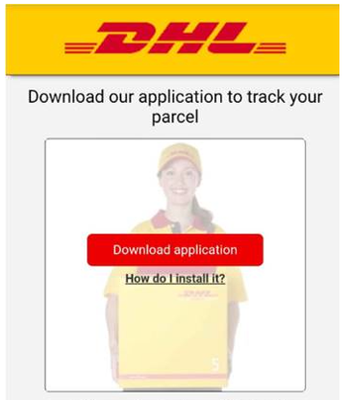
\includegraphics[scale=0.61]{dhl.png}
 \footnote{{Barabosch | 2021}}
\end{center}
\begin{center}
\begin{footnotesize}
 Abbildung 1: Beispiel einer Webseite nach aufruf des bösartigen Links.
 \end{footnotesize}
 
\end{center}
\newpage
\subsection{Post Infection}
Erste Handlung der Malware ist es nun, eine Verbindung zu dem Command and Control Server(C\&C) aufzubauen. Dieser kann als Hauptzentrale der Malware Infrastrukur bezeichnet werden. Von hier aus werden die Abläufe der Angriffe gesteuert. Auch gekaperte Daten werden hier in Datenbanken verschlüsselt gespeichert und weiterverabreitet. Ist die Verbindung hergestellt, durchsucht Flubot das komplette Adressbuch des infizierten Gerätes und sendet die Kontakte an den C\&C  Server. Dieser antwortet erneut mit einer Liste von Handynummern die bereits durch andere Bots gesichert wurden. Über diese wird nun die Verbeitung der Malware fortgesetzt. Um eine Mustererkennung und Blockierung vorzubeugen, verbreitet sich das Botnetz meist nur über neue Kontakte des C\&C Servers.\footnote{{Winter | 2021}}
\begin{center}
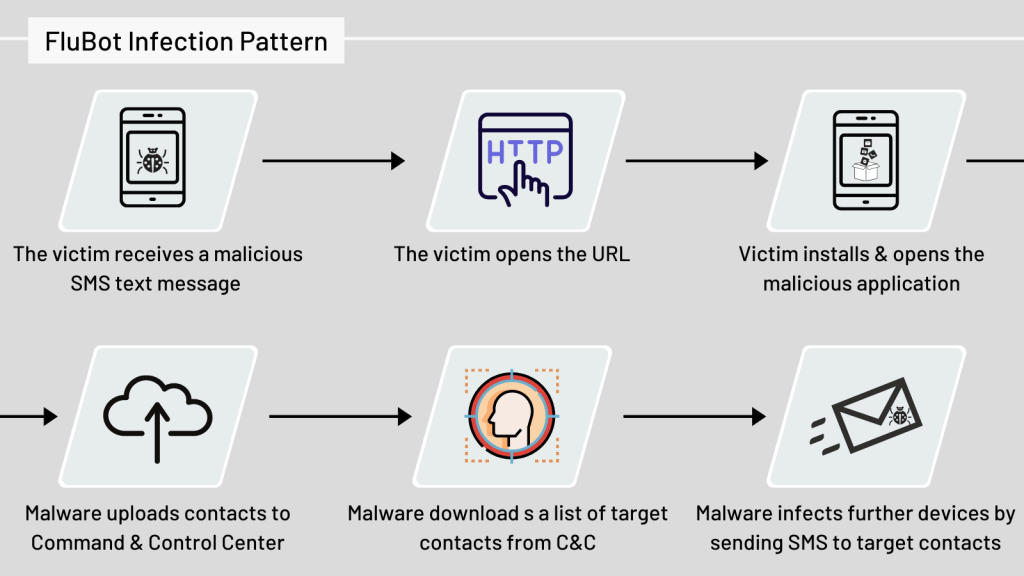
\includegraphics[scale=0.41]{command_control_server.png}\footnote{{threadmark.com | 2021}}
\end{center}
\begin{center}
\begin{footnotesize}
Abbildung 2: Ablauf einer Flubot Infektion

\end{footnotesize}
\end{center}
Des Weiteren schickt das infizierte Gerät eine Liste der installierten Applikationen an den Command and Control Server. Dieser antwortet wiederum mit einer Liste von Apps die kom­pro­mit­tie­rt werden sollen. Größtenteils konzentriert sich Flubot auf Banking Apps, aus denen Login Informationen ausgelesen werden. Weitere Ziele sind Dienste für Kryptowährungen. Darunter auch sogenannte Multi-Asset-Broker. Darunter versteht man Dienstleister, die den Handel mehrerer Vermögenswerte wie Aktien, ETFs oder auch Kryptowährungen anbieten. In allen Fällen werden die ausgewählten Anwendungen infiziert. Öffnet ein Opfer nun eine der betroffenen Apps, liegt ein Phishing Overlay des Login Screens als Maske über der eigentlichen Anwendung.
Jegliche Eingaben werden nun an den C\&C Server weitergeleitet.
Eine Zusammenfassende Darstellung lässt sich Abbildung 2 entnehmen.
Weitere schädliche Aktionen beinhalten das Deinstallieren von Apps, die Unterbindung von Benachrichtigungen und das Auslesen von Kreditkarten Informationen. Durch die Möglichkeit über den Command and Control Server immer wieder auch neue Angriffe zu steuern bietet Flubot über den ursprünglichen Nutzen hinaus die Möglichkeit Profit aus dem infizierten Gerät zu generieren.



\newpage
\section{Technische Analyse}
\subsection{Netzwerkstrukur}
Hinter Flubot steckt eine großflächige Infrastrukur. Kern des Ganzen bildet bekanntlich der Command and Control Server. Dieser liegt nicht fest auf einem Webspace, sondern arbeitet als verteiltes System auf mehreren hundert Instanzen. Kompromittierte Webseiten wie Wordpress Blogs dienen hierbei als Hosts. In früheren Botnetzen lag der C\&C Server fest auf einer dedizierten Domäne. Dies war einfach zu bekämpfen, da nach Ermittlung der IP Adresse der Internet-Service-Provider diese blockieren konnte und somit die Verbreitung des Botnetzes stoppte. Flubot entgegnet diesen Maßnahmen einmal durch die große Menge an Host-Servern und anhand des Domain Generation Algorithmus.\footnote{\Cite{threatmonit.com | 2021}} 
Dieser Algorithmus generiert dynamisch neue Domänennamen und versucht diese aufzulösen. Grob beschrieben bedient sich der Algorithmus aus einer Liste mit möglichen Top level Domains und generiert durch eine weitere Liste potenzielle second-level- Domains. Analysiert man den ausgehenden Netzwerkverkehr (vgl. Abbildung 3) eines infizierten Gerätes, so ist auffällig, dass teilweise bis zu 10 DNS Requests benötigt werden, bis eine auflösbare Domäne gefunden ist. Derzeit wird DNS über HTTPS für die Domäinauflösung verwendet. Dafür werden unter anderem Services wie dns.google oder cloudflare-dns.com genutzt.\footnote{{threatmonit.com | 2021}}
\begin{center}
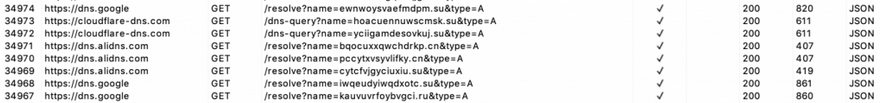
\includegraphics[scale=0.51]{dns.png}\footnote{threatmark.com | 2021}
\end{center}
\begin{center}
 \begin{footnotesize}
  Abbildung 3: Ausgehende DNS Requests
 \end{footnotesize}

\end{center}

Der gesamte Source Code der dies möglich macht liegt in der heruntergeladenen APK. In späteren Versionen wurde die eigentliche Payload in  Form der Phishing Malware erst nachträglich über den C\&C geladen. Hierbei wird ein GET-Request für die benötigten Dateien gestellt. Jegliche Kommunikation zwischen Gerät und Server wird zudem anhand von RSA verschlüsselt.
\newpage
\subsection{Payload}
Die Payload sowie die restliche APK von Flubot sind komplett in JAVA geschrieben. Sie enthält den benötigten Source Code um Kontakt zu dem C\&C Server herzustellen, die benötigten Berechtigungen einzufordern und die Phishing Malware auf ausgewählte Applikationen anzuwenden. Auch die RSA-Keys für die verschlüsselte Kommunikation sind enthalten. Die gepackte APK, welche den Payload trägt, ist anhand des MD5 Algorithmus gehashed und wird erst auf dem Gerät entpackt. Derzeit sind Geräte ab Android-Version 4.1.2 betroffen.\footnote{{bsi.de | 2020}}\\
Genauer betrachtet ist ein Android Application Package die  Installationsdatei für eine Android App. In ihr befinden sich alle benötigten Dateien für die Installation und Ausführung der Anwendung. In Grunde genommen ist eine Apk eine komprimierte zip Datei die auch mit bekannter Entpackungssoftware geöffnet werden kann. Das Gleiche gilt für Flubot. Um Sicherheitsanalysen jedoch zu erschweren verwendet die Malware sogenannte String Obfuscation. Dies ist ein Konzept, dessen Hauptaufgabe darin besteht, Programmcode zu verschleiern bzw. unleserlich zu machen. Dies wird beispielweise durch Variablensubstiution erreicht. Teilweise werden auch komplette Codeabschnitte verschlüsselt.\footnote{prodaft | 2021} Für die Obfuscation verwendet Flubot das Open Source tool paranoid.\footnote{Rocks | 2021}
Durch Reverse Engineering gelang es den Code zu Deobfuscieren, also wieder leserlich zu machen. 
Die Datei 'AndroidManifest.xml' (vgl. Beispiel 3) enthält alle Berechtigungen die eine APK benötigt. Flubot hat über 40 Einträge, die unter anderem Internet Zugriff und das Versenden von SMS autorisieren. 
\begin{shaded}
 android.permission.READ\_CONTACTS\\
 permission.WRITE\_SMS\\
 permission.INTERNET\\
 android.permission.READ\_PHONE\_STATE\\
 android.permission.QUERY\_ALL\_PACKAGES\\ 
 android.permission.WAKE\_LOCK\\ 
 android.permission.FOREGROUND\_SERVICE\\ 
 android.permission.REQUEST\_IGNORE\_BATTERY\_OPTIMIZATIONS\footnotemark


\end{shaded}
\footnotetext{threatmonit.com | 2021}
\begin{center}
 \begin{footnotesize}
  Beispiel 3: Berechtigungen in der Datei AndroidManifest.xml
 \end{footnotesize}

\end{center}

\newpage
Des Weiteren ist es gelungen, die Kommunikationskommandos zwischen Gerät und des Command and Control Servers zu erfassen. Derzeit sind über 20 Kommandos möglich, wobei Flubot stetig weiterentwickelt und um Funktionalitäten ergänzt wird. In Beispiel 4 ist ein Ausschnitt mit den häufigsten Kommandos des C\&C zu sehen.  \footnote{\Cite{Bilal | 2021}}

\begin{shaded}
GET\_CONTACTS - Schicke Kontakte an den Server\\
RETRY\_INJECT - Versuche erneut die Anwendung zu infizieren\\
BLOCK - Jegliche Kommunikation blocken\\
UNINSTALL\_APP - Deinstalltion der Malware\\
SEND\_SMS - Versenden von SMS\\
DISABLE\_PLAY\_PROTECT - Den Virenschutz des Google-Play-Stores deaktivieren\footnotemark
\end{shaded}
\footnotetext{Bilal | 2021}
\begin{center}
 \begin{footnotesize}
  Beispiel 4: Kommandos von C\&C Server an das infizierte Gerät
 \end{footnotesize}

\end{center}
Auch das infizierte Gerät ist in der Lage Kommandos zu versenden. Nachfolgend ein Beispielhafte Auswahl von Befehlen des Gerätes an den C\&C Server.

\begin{shaded}
GET SMS - Fordere Phishing SMS und Mobilfunknummer an\\
GET INJECTS LIST - Erhalte eine Liste der Zielanwendungen und sende die zugehörigen Paketnamen\\
GET INJECT - Fordert den HTML-Code für das jeweilige Phishing Overlay an.\\
SMS\_RATE - Festlegung der zu verschickenden Phishing SMS\footnotemark
\end{shaded}
\footnotetext{Bilal | 2021}
\begin{center}
 \begin{footnotesize}
  Beispiel 5: Kommandos von Gerät an C\&C Server
 \end{footnotesize}

\end{center}

\newpage
Die eigentliche Phishing Attacke, welche ein Overlay über die betroffene Anwendung legt, wird mittels Webview umgesetzt. Das heißt, bei Öffnung der infizierten App, wird das Overlay mittels HTML-Code im Browser dargestellt und über die Anwendung gelegt.\footnote{scamwatch.gov.au | 2021}
\begin{shaded}
\begin{internallinenumbers}
 \begin{lstlisting}
 private void LoadHtml() {
  String GetInject = Bot.GetInject(packagename);
  #package name wird durch die geziele Application ersetzt.
   if (GetInject==0) {
	finishandRemovetask();
	 }   else {
	this.webView.loadDataWithBaseURL(null, GetInject,
	Deobfuskator$app$Release.getString(-225216466544654L);
	Deobfuskator$app$Release.getString(-225216466544654L);
	null;
	)
 }
 }
\end{lstlisting}
\end{internallinenumbers}

\hspace{15cm}\footnotemark
\end{shaded}
\footnotetext{threatmonit.com | 2021}
\begin{center}
 \begin{footnotesize}
  Codebeispiel 1: Der Deobfuscierte Source-Code einer Funktion die das Phishing Overlay über die gezielte Anwendung legt
 \end{footnotesize}

\end{center}
In Zeile 2 von Codebeispiel 1 ist zu sehen, wie die Variable 'packagename' als Parameter für die Funktion GetInject übergeben wird. In Zeile 7 wird das Phishing Overlay durch die Funktion 'webView' geladen. Flubot wird stetig weiterentwickelt und gewinnt zunehmend an Komplexität. Technisch ist die Malware auf dem neuesten Entwicklungsstand und auch aufgrund der Größe höchstwahrscheinlich von einem größeren Team professionell entwickelt worden.  




\newpage
\section{Lösungsansätze}
Flubot hat einige Mechanismen implementiert um nicht identifiziert und entfernt zu werden. So wird die Anwendung nicht unter installierter Software gelistet und ist auch in einigen Taskmanagern nicht als Prozess sichtbar. Findet man die Installationsdatei dennoch, blockiert Flubot den Android Deinstaller. Des Weiteren ist Flubot in der Lage 'Play protect' zu deaktivieren. Dennoch ist die Entfernung der Malware durch Rücksetzung des Smartphones zum Werkzustand recht einfach.\footnote{\Cite{threatmonit.io | 2021/}} Dies hat allerdings ein Verlust der persönlichen Daten zur Folge. Eine Entfernung ohne Datenverlust ist beispielweise durch das Open-Source tool 'malninstall'\footnote{Github/linuxct | 2021} möglich. Dieses Tool wurde speziell für die Entfernung von Flubot entwickelt.\\
Grundsätzlich gibt es keine generelle technische Lösung gegen Phishing Malware. Da solch Angriffe in erster Linie Social Engineering nutzen, ist es schwierig eine technische Lösung dagegen zu entwickeln. Der Mensch ist immer der anfälligste Teil eines sicherheitsrelevanten Systems. Einen gewissen Schutz bietet jedoch Zwei-Faktor-Authentifizierung, der wenn möglich in allen Anwendungen aktiviert sein sollte\\ Das präventiv größtmögliche Potential stellt eine bessere Bildung und Aufklärung der Gesellschaft dar. Informatik sollte in Schulen deutlich stärker gewichtet werden und auch IT- sicherheitsrelevante Themen lehren. Des weiteren sollte der Grundsätzliche Medienumgang in Bildungseinrichtungen stärker in den Fokus gerückt werden. 
\newpage
\section{Conclusion}
Phishing ist nach wie vor die meist verwendete Methode um sicherheitsrelevante Daten abzugreifen. Solange der Endnutzer nicht über die notwendige Expertise verfügt, um derartige Angriffe zu erkennen und abzuwehren wird Phishing Malware auch in Zukunft eine große Rolle spielen.\\
Durch neue Technologien wie das 'Internet der Dinge' wird die Menge der angreifbaren Ziele immer weiter steigen. Die einzige Möglichkeit nachhaltig dem Problem entgegenzuwirken stellt eine ausreichend frühe Aufklärung hinsichtlich digitaler Angriffsszenarien dar.\\
Die Drahtzieher hinter Flubot wurden im Herbst 2021 in Spanien festgesetzt.\footnote{ Cimpanu | 2021} Zum Stand dieser Arbeit verbreitet sich das Botnetz allerdings nach wie vor. 

\newpage
\section{Eigentständigkeitserklärung}
Hiermit bestätige ich, dass ich die vorliegende Arbeit selbstständig verfasst und keine anderen Publikationen als die angegebenen benutzt habe. Alle Teile meiner Arbeit, die wortwörtlich oder dem Sinn nach anderen Werken entnommen sind, wurden unter Angabe der Quelle kenntlich gemacht. Gleiches gilt für von mir verwendeten Internetquellen. Die Arbeit ist weder von mir noch von einem Kommilitonen in einem anderen Seminar vorgelegt worden.\\
Moritz Rupp, Albstadt, 07.01.2022
\newpage
\section{Literaturverzeichnis}
\footnotesize
1 | statista, 15.06.2021,  Anzahl der in Gebrauch befindlichen Smartphones weltweit in den Jahren 2019 und 2020 und Prognose bis 2022 https://de.statista.com/statistik/daten/studie/1235321\\

2 | statista, 11.10.21 Statistiken zu Android, https://de.statista.com/themen/1355/android/\\

3 | Thomas Barabosch, 14.09.2021, Flubot’s Smishing Campaigns under the Microscope, https://www.telekom.com/en/blog/group/article/flubot-under-the-microscope-636368\\

4 | Thomas Barabosch, 14.09.2021, Flubot’s Smishing Campaigns under the Microscope, https://www.telekom.com/en/blog/group/article/flubot-under-the-microscope-636368\\

5 | Andy Voß, 04.10.2021, Flubot: Android-Malware verbreitet sich über Fake-Patches,https://www.computerbild.de/artikel/cb-News-Sicherheit-Flubot-Gefaehrliche-Android-Malware-verbreitet-sich-ueber-Fake-Patches-30863335.html\\

6 | Jens Stark, 13.09.2021, Android-Malware FluBot stürmt Top-ten, https://computerwelt.at/news/android-malware-flubot-stuermt-top-ten\\

7 | L.Warner, 09.04.2021, Major Data Breach at Facebook this week, https://wa.rner.me/2021/04/09/major-data-breach.html\\


8 | Thomas Barabosch, 14.09.2021, Flubot’s Smishing Campaigns under the Microscope, www.telekom.com/en/blog/group/article/flubot-under-the-microscope-636368\\

9 | Thomas Barabosch, 14.09.2021, Flubot’s Smishing Campaigns under the Microscope, www.telekom.com/en/blog/group/article/flubot-under-the-microscope-636368\\

10 | Thomas Barabosch, 14.09.2021, Flubot’s Smishing Campaigns under the Microscope, www.telekom.com/en/blog/group/article/flubot-under-the-microscope-636368\\

11 | Luca Winter, 20.05.2021, FluBot Malware – All You Need to Know \& to Act Now, https://www.threatmark.com/flubot-banking-malware\\

12 | threadmark.com, 20.05.2021,FluBot Malware – All You Need to Know \& to Act Now, https://www.threatmark.com/flubot-banking-malware\\

13 | threadmonit.io, 16.08.2021,FluBot Android Malware Technical Analysis, https://www.threatmonit.io/flubot-android-malware-technical-analysis, https://www.threatmark.com/flubot-banking-malware\\

14 | threadmonit.io, 16.08.2021,FluBot Android Malware Technical Analysis, https://www.threatmonit.io/flubot-android-malware-technical-analysis, https://www.threatmark.com/flubot-banking-malware\\

15 | threadmark.com, 20.05.2021,FluBot Malware – All You Need to Know \& to Act Now, https://www.threatmark.com/flubot-banking-malware\\

16 | bsi.de, https://www.bsi.bund.de/DE/Themen/Verbraucherinnen-und-Verbraucher/Cyber-Sicherheitslage/Methoden-der-Cyber-Kriminalitaet/Botnetze/Steckbriefe-aktueller-Botnetze/Steckbriefe/Flubot.html\\

17 | github.com/prodaft, 15.07.2021, https://github.com/prodaft/malware-ioc/tree/master/FluBot\\

18 | Michael Rocks, 02.12.2021, https://github.com/MichaelRocks/paranoid\\

19 | threadmonit.io, 16.08.2021,FluBot Android Malware Technical Analysis, https://www.threatmonit.io/flubot-android-malware-technical-analysis, https://www.threatmark.com/flubot-banking-malware\\

20 | Ahmed Bilal, 10.11.2020, Flubot Malware Analysis Report, https://github.com/prodaft/malware-ioc/blob/master/FluBot/FluBot.pdf\\

21 | Ahmed Bilal, 10.11.2020, Flubot Malware Analysis Report, https://github.com/prodaft/malware-ioc/blob/master/FluBot/FluBot.pdf\\

22 | Ahmed Bilal, 10.11.2020, Flubot Malware Analysis Report, https://github.com/prodaft/malware-ioc/blob/master/FluBot/FluBot.pdf\\

23 | scamwatch.gov.au, 06.10.2021, Missed delivery, call or voicemail (Flubot) scams, https://www.scamwatch.gov.au/news-alerts/missed-delivery-call-or-voicemail-flubot-scams\\

24 | threadmonit.io, 16.08.2021,FluBot Android Malware Technical Analysis, https://www.threatmonit.io/flubot-android-malware-technical-analysis\\

25 | threadmonit.io, 16.08.2021,FluBot Android Malware Technical Analysis, https://www.threatmonit.io/flubot-android-malware-technical-analysis, \\

26 | github.com/linuxct | 13.05.2021, https://github.com/linuxct/malninstall\\

27 | Catalin Cimpanu | 16.04.2021, Despite arrests in Spain, FluBot operations explode across Europe and Japan, https://therecord.media/despite-arrests-in-spain-flubot-operations-explode-across-europe-and-japan/
\printbibliography
\end{document}

